\documentclass[../CourseManual.tex]{subfiles}

\begin{document}

Lloyd's algorithm takes a system of agents and allocates them evenly over an area according to the distribution of some resource of interest. This could be applied to search and rescue missions, robots collecting soil samples, or other situations where agents must cover some limited area and so they spread out to service it. 
\subsection{Lloyd's Algorithm Dynamics} \label{Lloyd Dynamics}
Lloyd's algorithm is distinct from the previous algorithms' mathematics. This algorithm is better suited to model distributed convergence rather than convergence to a location or velocity. The following sections explain each component of Lloyd's algorithm in detail.

\subsubsection{Density} \label{Lloyd Density}
Lloyd’s algorithm allocates agents to optimal positions over a fixed area, $A \subset \mathbb{R}^2$, to maximize coverage of some density, $D : A \rightarrow \mathbb{R}_{\geq0}$. $D$ may be either constant or time-variant. The range of $D$ must be non-negative as density is non-negative by definition, and the simulation will behave unexpectedly otherwise. \\

Example - Constant Density: Search and Rescue \\

Consider a scenario where robotic agents are tasked with exploring an area in search of multiple target objects. In this situation, the density of the area which we are trying to optimize our coverage of could be represented as a constant probability distribution map in the form of a matrix where cell $(i,j)$ represents the probability of the presence of a target object at the cell's corresponding location in $A$. \\ 

Example - Time Variant Density: Wildfire Suppression \\

Consider a scenario where robotic agents are tasked with suppressing a growing wildfire through the use of a retardant dispersal system. In this situation, the density of the area which we are trying to optimize our coverage of could be represented as a time-variant heat map in the form of a function, $D(x,y,t)$, which takes in $x$ and $y$ coordinates as well as the time $t$ and returns the heat intensity of location $(x,y)$ at time $t$ \\

For more detail on density and how to implement it in MATLAB, read \hyperref[Matrix Editor: Lloyd]{Section \ref{Matrix Editor: Lloyd}}. 

\subsubsection{Agents} \label{Lloyd Agents}
For $n$ agents, we denote the set of all agents as $V \:(|V | = n)$. Let each agent be denoted $v_i \in V$, the position of each $v_i$ be $p_i \in P$ for each $i \in \{1, . . . , n\}$, where $P \subset A$ is the set of all agent positions.

\subsubsection{Communication} \label{Lloyd Communication}
Lloyd's algorithm takes into account a radius of communication, $r_c$. If agent $v_j$ is at $p_j$, and $p_j$ is within $r_c$ of agent $v_i$'s position $p_i$ (i.e. $p_j \in \bar{B}_{r_c}(p_i)$), then $v_i$ and $v_j$ can communicate with one another. Note that communication goes both ways, i.e. if $v_i$ can communicate with $v_j$, then $v_j$ can communicate with $v_i$. More formally, if $v_i$ and $v_j$ are in the same communication graph (i.e. there exists a path between $v_i$ and $v_j$), they can communicate. By doing this, we partition $V$ into sets of agents that can communicate with each other. Denote these sets $V_k \subseteq V, k \in \{1, . . . , K\}$, where $K$ is the number of disjoint communication graphs. 

\subsubsection{Observation} \label{Lloyd Observation}
Lloyd's algorithm also takes into account a radius of observation $r_o$. Agent $v_i$ at position $p_i$ observes all the points within $r_o$ of $p_i$. Formally, agent $v_i$ observes the region $\bar{B}_{r_o}(p_i)$. Moreover, we assume agents in the same communication graph share information about their observed regions and the density within them. Let $O_k \subseteq A$ be the observed region by all agents in $V_k$, then  
\[O_k = \bigcup_{i} \bar{B}_{r_o}(p_i),\; i \in V_k.\]
Then, we determine the points in $O_k$ which are closest to each agent $v_i$, $i \in V_k$. This partitions $O_k$ into Voronoi regions. Let $R_{k_i} \subseteq O_k$, $i \in V_k$ be such partitions. We then have
\[R_{k_i} = \{x \in O_k : \| x - p_{i_k} \| \leq \| x - p_{j_k} \| \ \forall j \in V_k\}.\]
Agent $v_i$ is then assigned the partition $R_{k_i}$. The above process is repeated for each $k \in \{1, . . . , K\}$, and thus each agent $v_i$ is assigned a region $R_{k_i}$. Note that in some cases, $\bigcap_{k=1}^K O_k \neq \emptyset$, and $\bigcup_{k=1}^K O_k \neq A$ (i.e there may be some overlap in coverage and not complete coverage of the target area, respectively).

\subsubsection{Convergence} \label{Lloyd Convergence}
Each agent then converges to the centroid of their assigned region. This is done by calculating the mass $M_{k_i} \in \mathbb{R}$ of each region $R_{k_i}$ using
\[M_{k_i} =\int_{R_{k_i}}D(x, y)dA,\]
and the centroid $C_{k_i} \in A$ of $R_{k_i}$ is given by
\[C_{k_i} =\frac{1}{M_{k_i}}\left(\int_{R_{k_i}} x \cdot D(x, y)dA, \int_{R_{k_i}} y \cdot D(x, y) dA\right).\]

\subsubsection{Movement} \label{Lloyd Movement}
Finally, the agent $v_i$ will move towards their $C_{k_i}$. The centroid of each region is effectively a weighted average position, so the net effect is that agents will disperse over $A$ to maximize the mass of their observed regions.

\subsubsection{Limitations} \label{Lloyd Limitations}
In practice, few resources can be described with a continuous density function. Even if this were possible, it is not feasible to compute integrals to a high precision in real time. Instead, the integrals above are computed by discretizing the density functions and taking sums. This improves computation time at the cost of accuracy. \\

If density is time-invariant, agents will converge at $C_{k_i}$. This is the optimal positions for the agents to maximize the mass of their observed regions. Note that this heavily depends on $r_o$, $r_c$, and $D$. If $r_c < r_o$, the agents may not know that they are covering the same area. If $r_o$ is sufficiently small and $D$ has local maximums, then an agent may converge to a less-than-optimal $C_{k_i}$. \\



\subsection{Simulation App} \label{Simulation App: Lloyd}
Upon first glance, the simulation app for Lloyd's algorithm can appear very intimidating. Don't be alarmed. This is your guide to understanding all components. 

%app picture goes before the descriptions
\begin{figure}[H]
    \centering
    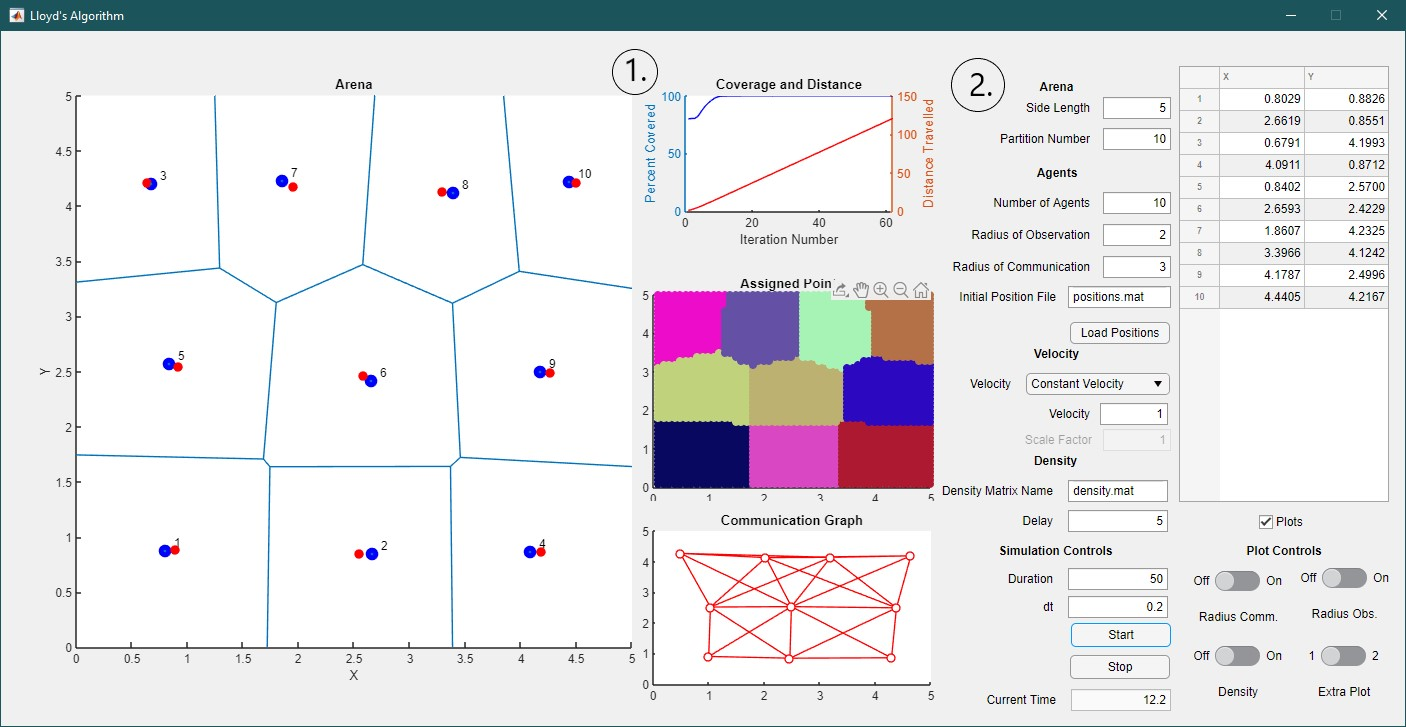
\includegraphics[width=350pt]{media/Lloyd.jpg}
    \caption{Screen capture of LloydApp.mlapp with default settings}
    \label{fig: lloyd app}
\end{figure}

\subsubsection{Plots} \label{Lloyd Plots}
Area 1 of Figure \ref{fig: lloyd app} displays the plots section of the Lloyd app. This section contains four separate plots: the \textbf{Arena} plot, the \textbf{Coverage and Distance} plot, the \textbf{Assigned Points} plot, and the \textbf{Communication Graph} plot. \\

The \textbf{Arena Plot} displays agent positions as \textcolor{blue}{blue dots}, region centroids as \textcolor{red}{red dots}, and a Voronoi diagram to illustrate each agent's assigned region. In the \textbf{Plot Controls} section, a contour diagram can be toggled to display density information, and observation radii can be toggled to display observation circles around each agent. \\

The \textbf{Coverage and Distance} plot displays coverage of the arena's density as a percentage of total unique observed mass over total arena mass on the left axis, in \textcolor{blue}{blue}. On the right, the cumulative distance travelled by all agents is shown in \textcolor{red}{red}. The independent axis for both plots is time, measured in iterations. \\

The middle plot (by default, \textbf{Assigned Points} plot) can be configured to display two different plots. Plot 1 displays all discrete points assigned to each agent in a different colour. Plot 2 displays each agent's energy on a bar graph. This is useful if your agents' energy supply (battery, fuel level, etc.) drains as they move. The plot can be switched during the simulation in the \textbf{Plot Controls} section. \\

The \textbf{Communication Graph} plot displays one or more un-directed graphs to show which agents are in communication. In the \textbf{Plot Controls} section, communication radii can be toggled to display communication circles around each agent. \\

The \textbf{Agent Position Table} displays the current position of each agent throughout the simulation. Before the simulation starts, you can manually edit positions using this table. You can also load predefined positions for arbitrary agents into the table (see \hyperref[Lloyd Agent Controls]{Section \ref{Lloyd Agent Controls}}).

\subsubsection{User Controls} \label{Lloyd Controls}
Area 2 of Figure \ref{fig: lloyd app} displays the user controls section of the Lloyd app. This section is divided into 5 sub-sections: the \textbf{Arena} sub-section, the \textbf{Agents} sub-section, the \textbf{Velocity} sub-section, the \textbf{Density} sub-section, and the \textbf{Simulation Controls} sub-section. \\

In the \textbf{Arena} sub-section, you can specify physical dimensions of your simulation arena in the \textbf{Side Length} field. Additionally, each physical unit can be subdivided into multiple partitions for higher simulation resolution in the \textbf{Partitions} field. Note that the simulation arena must be a square. For example, if you want to simulate a 10m-by-10m arena with accuracy to 0.5m, you would specify a \textbf{Side Length} of 10 and \textbf{Partitions} of 2. \\

\label{Lloyd Agent Controls}
In the \textbf{Agents} sub-section, you can specify the \textbf{Number of Agents} for the simulation, the \textbf{Radius of Observation} for all agents, and the \textbf{Radius of Communication} for all agents. Note that changing the \textbf{Number of Agents} field will change the number of rows in the \textbf{Agent Position Table}. If you want to load initial positions from a \textit{.mat} file, specify the file name (including the file extension) and press the \textbf{Load Positions} button. This will overwrite the \textbf{Agent Position Table} data and the \textbf{Number of Agents} field. \\

The \textbf{Velocity} sub-section allows you to change how agents move. If \textbf{Velocity Type} is Constant, agents will move the specified distance in the \textbf{Velocity} field every iteration. If \textbf{Velocity Type} is Proportional, agents will move at a velocity proportional to the distance to their centroid times the \textbf{Scale Factor}. Agents will not exceed \textbf{Maximum Velocity} in Proportional Velocity mode. \\

The \textbf{Density} sub-section allows you to specify the name (including the \textit{.mat} extension) of your density file. Density will be loaded from the file when the simulation begins. You must create a density file using the \textbf{Matrix Editor}. The \textbf{Delay} field specifies the how often $D$ will be updated. Delay is only useful if your density is time-variant. \\

The \textbf{Simulation Controls} sub-section contains: the \textbf{Duration} field to select the length of time for which your simulation will run; the \textbf{dt} field to select the simulated time step $\Delta t$; the \textbf{Start} and \textbf{Stop} buttons to begin and end your simulation, respectively. The \textbf{Current Time} field displays the simulation's current time. The \textbf{Plots} checkbox, when enabled, will update selected plots and tables. Disabling \textbf{Plots} will greatly increase the speed of your simulation. This is useful if you need to simulate for more than a few hundred iterations.

\subsubsection{Matrix Editor} \label{Matrix Editor: Lloyd}

The \textbf{Matrix Editor Lloyd} app serves two purposes: to create your density matrix/function, and to create your initial agent position matrix. \\

\begin{figure}[H]
    \centering
    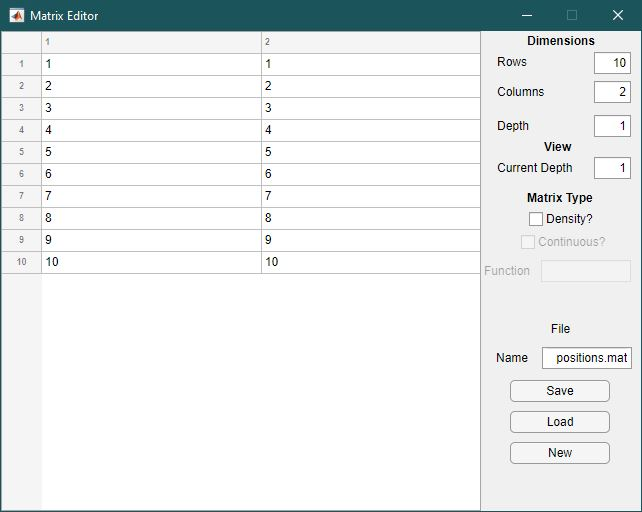
\includegraphics[width=350pt]{media/MatrixEditorLloyd.JPG}
    \caption{Screen capture of MatrixEditorLloyd.mlapp with default position settings}
    \label{fig: matrix editor lloyd}
\end{figure}

\textbf{Density:}
\begin{enumerate}
    \item Ensure you have determined a density that models your topic, i.e. on paper. You must thoroughly consider this step, otherwise your simulation results will not accurately model your topic
    \item Check the \textbf{Density?} box
    \item Depending on your density, do one of the following:
    \begin{enumerate}[label=(\alph*)]
        \item If your density is a continuous function $D(x,y,t)$, check the \textbf{Continuous?} box and enter the expression in the \textbf{Function} field. Ensure that $D(x,y,t) \geq 0$ for all $(x,y) \in A$ and $t \in [0, duration]$
        \item If your density is comprised of discrete constant values or discrete functions of $t$, the density matrix will be a square matrix with side lengths of $sides \times partitions$ where $sides$ is the side length of the arena and $partitions$ is the partition number of the arena. i.e., if the arena dimension is 2km $\times$ 2km and the partition number is 4, then both \textbf{rows} and \textbf{columns} should have a value of 8 such that the density matrix is an  $8 \times 8$ matrix.
        \item If you need more complex density behaviour, ask a TA for help
    \end{enumerate}
    \item When you're done, specify a file name (including the \textit{.mat} extension) and press the \textbf{Save} button
\end{enumerate}

\textbf{Agent Positions:}
\begin{enumerate}
    \item Specify the number of agents you would like in the \textbf{Rows} field
    \item Set \textbf{Columns} to 2
    \item Enter the initial positions for each agent in the grid. Column 1 is X, column 2 is Y
    \item When you're done, specify a file name (including the \textit{.mat} extension) and press the \textbf{Save} button
\end{enumerate}
If you're finished editing one file, and would like create another, press the \textbf{New} button. If you need to edit a file, specify the proper file name and press the \textbf{Load} button. Be sure to save your changes.


\subsubsection{Parameters and Variables}

\renewcommand{\labelenumi}{\roman{enumi}}
\begin{enumerate}
  \item Side Length $(sides)$: Dimensions of A, which is restricted to a square region. Hence, A is an area with dimensions $sides \times sides$. The units of these dimensions is determined by the user.
  
  \item Partition Number $(partitions)$: The space A is discretized by dividing each unit of space by $Partition Number$ where $Partition Number \in \mathbb{Z}_{>0}$. For example, if $A$ has dimensions $5 \times 5$ and $Partition Number = 10$, then $A$ is represented in MATLAB by a $50 \times 50$ matrix.
  
  \item Density $(density)$: Once the space is discretized, a density matrix is created with dimensions $sides \cdot Partition Number \times sides \cdot Partition Number$. A cell $(x,y) \in A$ can be mapped to its associated cell $(i,j) \in density$ with
  
  $$(i,j) = (floor(x \cdot Partition Number), floor(y \cdot Partition Number)),$$
  
  similarly, a cell $(i,j) \in D$ can be mapped to its associated cell $(x,y) \in A$ with
  
  $$(x,y) = (\dfrac{i}{Partition Number},\dfrac{j}{Partition Number}).$$
  
  \item Agent Positions $(agentPositions)$: An $N \times 2$ matrix with the x-position of agent $v_i$ in the first column of row $i$, and the y-positions in the second column, as below:
  
  $$Agent Positions = 
  \begin{bmatrix}
    p_{1_{x}} \hspace{0.5cm} p_{1_{y}}\\
    p_{2_{x}} \hspace{0.5cm} p_{2_{y}}\\
    \vdots \hspace{0.5cm} \vdots \\
    p_{N_{x}} \hspace{0.5cm} p_{N_{y}}\\
  \end{bmatrix}$$
  
  \item Adjacency Matrix $(adjMatrix)$: The $N \times N$ symmetric adjacency matrix:
  
  $$adjMatrix(i,j) = 
  \begin{cases}
    1, & \text{if agent $v_i$ communicates with agent $v_j$}\\
    0, & \text{otherwise.}
  \end{cases}$$
  
  \item Communication Cells $(commCells)$: The $1 \times K$ Cell array, where cell $k$ represents the communication group $V_{k}$ (see \hyperref[Lloyd Communication]{Section \ref{Lloyd Communication}}). Hence, the matrix looks as follows:
  
  $$agentPoints = 
  (\begin{bmatrix}
    v^{1}_{1}\\
    v^{1}_{2}\\
    \vdots\\
    v^{1}_{n}\\
  \end{bmatrix}, 
  \begin{bmatrix}
    v^{2}_{1}\\
    v^{2}_{2}\\
    \vdots\\
    v^{2}_{m}\\
  \end{bmatrix}, 
  \dots, 
  \begin{bmatrix}
    v^{K}_{1}\\
    v^{K}_{2}\\
    \vdots\\
    v^{K}_{p}\\
  \end{bmatrix})$$
  
  where $\bigcup_{i=1}^{K} V_{i} = V$
  
  \item Agent Points $(agentPoints)$: A $1 \times N$ cell array that contains $r \times 2$ matrices. Matrix $i$ contains the discretized points of $R_{k_{i}}$, hence $r$ is the number of points in $R_{k_{i}}$ (note that there is only a finite number of them since the space has been discretized). The first column of $agentPoints$ contains the x-coordinates, and the second column contains the y-coordinates. If the total number of points in each $R_{k_{i}}$ is $K_{i}$, then the matrix looks as follows:
  
  $$agentPoints = 
  (\begin{bmatrix}
    x_{1, v_{1}} \hspace{0.5cm}  y_{1, v_{1}}\\
    x_{2, v_{1}} \hspace{0.5cm}  y_{2, v_{1}}\\
    \vdots \hspace{0.5cm} \vdots \\
    x_{K_1, v_{1}} \hspace{0.5cm}  y_{K_1, v_{1}}\\
  \end{bmatrix}, 
  \begin{bmatrix}
    x_{1, v_{2}} \hspace{0.5cm}  y_{1, v_{2}}\\
    x_{2, v_{2}} \hspace{0.5cm}  y_{2, v_{2}}\\
    \vdots \hspace{0.5cm} \vdots \\
    x_{K_2, v_{2}} \hspace{0.5cm}  y_{K_2, v_{2}}\\
  \end{bmatrix}, 
  \dots, 
  \begin{bmatrix}
    x_{1, v_{N}} \hspace{0.5cm}  y_{1, v_{N}}\\
    x_{2, v_{N}} \hspace{0.5cm}  y_{2, v_{N}}\\
    \vdots \hspace{0.5cm} \vdots \\
    x_{K_N, v_{N}} \hspace{0.5cm}  y_{K_N, v_{N}}\\
  \end{bmatrix})$$
  
  %% REVIEW THIS %%
  
  \item Mass $(mass)$: A $1 \times N$ array containing the mass of $R_{k_{i}}$ in column $i$ where the mass is calculated with
  
  $$mass(i) = \sum_{(i,j)}density(x_i,y_i) \hspace{0.25cm} \forall \hspace{0.25cm} (x_i,y_i) \in R_{k_{i}}$$
  
  \item Centroids $(centroids)$: An $N \times 2$ matrix containing the x-position of the centroid of $R_{k_{i}}$ in the first column of row i and the y-position in the second column. The centroids are calculated with
  
  $$centroids(i,1) = \dfrac{1}{mass(i)}\cdot \sum_{(x_i,y_i)}x_i \cdot density(x_i,y_i) \hspace{0.25cm} \forall \hspace{0.25cm} (x_i,y_i) \in R_{k_{i}}$$
  
  $$centroids(i,2) = \dfrac{1}{mass(i)}\cdot \sum_{(x_i,y_i)}y_i \cdot density(x_i,y_i) \hspace{0.25cm} \forall \hspace{0.25cm} (x_i,y_i) \in R_{k_{i}}$$
  
  \item Percent of Covered Mass $(coverage)$: Ratio of the mass contained by points that are covered by an agent $(coveredMass)$ divided by the mass contained by the arena $(totalMass)$. A point $(x,y)$ is considered covered by agent $i$ if $(x,y) \in B_{r_{o}}$. 
  
  \item Velocity Scale Factor $(scaleFactor)$: This is used in the simulation if Velocity Type is set to Proportional Velocity. The user may have the agents move as follows: Given an agent in position $p_i$ and the centroid $C_{k_{i}}$ of the agent’s assigned region $R_{k_{i}}$, then in one iteration, agent $i$ will move a distance of $scaleFactor \cdot ||C_{k_{i}} - p_i||$. Note that $scaleFactor$ must be greater than zero in order for the agents to move, and less than 2 in order for the algorithm to converge. A $scaleFactor$ of 1.8 is generally accepted to lead to the fastest convergence, however this value may not be realistic given one’s application.
  
  \item Velocity $(velocity)$: Each iteration represents a time step of $\Delta t$. The units of space and time are determined by the user. For example, if you decide that each unit of space in the algorithm represents 1 km, and each unit of time is 1 hour, then velocity will be in units of km/h. Hence, after one iteration agent $i$ will have moved a distance of $\Delta t \cdot velocity$ in the direction of the centroid of $R_{k_{i}}$.
  
  \item Max Velocity $(maxVelocity)$: Once the distance d to move after one iteration is determined, the agent’s velocity is taken to be $v = \dfrac{d}{\Delta t}$. If $v > maxVelocity$, the velocity of the agent will be set to max velocity for that iteration. Note that if a constant velocity $v$ is implemented and $v < maxVelocity$, then max velocity has no effect on the algorithm.
  
  \item Delay $(delay)$: If your density is dynamic, i.e. it changes over time, then delay determines the number of iterations between each change. For example, if $delay = 5$, then $density$ will only change every $5^{th}$ iteration. Note that delay must be a natural number.
  
  \item Radius of Observation $(rObs)$: The radius of observation $r_o$ is defined such that an agent $v_i$ at position $p_i$ observes all the points within $r_o$ of $p_i$.
  
  \item Radius of Communication $(rComm)$: The radius of communication $r_c$ is defined such  agent $v_i$ at position $p_i$ communicates with all agents within $r_c$ of $p_i$.
  
  \item Number of Agents $(numAgents)$: Total number of agents $(N)$ used in simulation.
  
  \item Distance Travelled $(distanceTravelled)$: An array that contains the sum of the distances traveled by all agents each iteration.
  
  \item Energy $(energy)$: A $1 \times N$ array containing the energy of agent $i$ in column $i$. You must determine the units of the energy that you wish to use and how you want to represent this in the energy array. The energy will decrease after every iteration by some parameter (you may choose how to represent this). In the regular algorithm, we decrease the energy of each agent depending on the velocity they move at with
  
  $$energy(i)_{j+1} = energy(i)_j - \dfrac{1}{2}m_i v_i^2,$$
  
  where $m_i$ is the mass of the agent, $v_i$ is its velocity, and $j$ is the time step.
  
\end{enumerate}

\subsubsection{MATLAB Functions} \label{MATLAB Functions: Lloyd}
The following functions are external MATLAB functions. Most will need to be programmed by you, but some will be given. \\

\textbf{communication.m} -- communication.m is used to calculate which agents are in communication as seen in \hyperref[Lloyd Communication]{Section \ref{Lloyd Communication}}. The communication function takes inputs $agentPositions$ and $rComm$, and outputs $commCells$ and $adjMatrix$. $adjMatrix$ is calculated by looping through all agents $v_i$ and $v_j$ and setting $adjMatrix(i,j) = 1$ if they are within each others radius of communication. $comCells$ is calculated using MATLAB's graph function to create a graph of the adjacency matrix as well as MATLAB's conncomp function to return the connected components of the graph where $commCells(i)$ contains the agent IDs for all agents that belong to component $i$. \\

\textbf{assignAgentPoints.m} -- assignAgentPoints.m is used to assign points in the arena to agents based on the algorithm discussed in \hyperref[Lloyd Observation]{Section \ref{Lloyd Observation}}. Agents in the same communication cell should not be assigned the same points. However, agents who cannot communicate may cover the same points. The assignAgentPoints function takes inputs  $agentPositions$, $commCells$, $sides$, $partitions$, and $rObs$, and outputs $agentPoints$. $agentPoints$ is calculated by looping through each communication cell and using MATLAB's rangesearch function to determine which points in the arena are within each agent's radius of observation. \\ 

\textbf{calcMass.m} -- calcMass.m is used to calculate the total mass of each agent's observed region. The calcMass function takes inputs $agentPoints$, $density$, and $partitions$, and outputs $mass$. $mass$ is calculated by summing the density over each agent's observed region. \\

\textbf{calcCoverage.m} -- calcCoverage.m is used to calculate how much of the total mass in the arena is being observed by the agents. The calcCoverage function takes inputs $agentPoints$, $partitions$, $density$, and $totalMass$, and outputs $coverage$. $CalcMass$ is calculated by summing the density over each agent's observed region and dividing by the total mass in the arena. \\

\textbf{calcCentroids.m} -- calcCentroids.m is used to calculate the centroid of each agent's observed region as discussed in \hyperref[Lloyd Convergence]{Section \ref{Lloyd Convergence}}. The calcCentroids functions takes inputs $agentPoints$, $mass$, $density$, $agentPositions$, and $partitions$, and outputs $centroids$. $centroids$ is calculated by looping through each agent and taking the weighted average of the points in their observed region based on the points' masses. \\

\textbf{moveAgents.m} -- moveAgents.m is used to calculate the movement of each agent towards its centroid, as described in \hyperref[Lloyd Movement]{Section \ref{Lloyd Movement}}. Additionally, this function updates the distance travelled statistic and agent energy levels. The moveAgents function takes inputs $agentPositions$, $centroids$, $sides$, $dt$, $energy$, $velocityType$, $maxVelocity$, and $scaleFactor$, and outputs the updated $agentPositions$, $distanceTravelled$, and $energy$. $agentPositions$ is updated by calling the velocityFunction function to determine the positional change of each agent and adding the change to $agentPositions$. $distanceTravelled$ is updated by calculating and summing the distance travelled by each agent. $energy$ is updated by calling the energyFunction function to determine the energy change of each agent and adding the change to $energy$. \\

\textbf{velocityFunction.m} -- velocityFunction.m is used to calculate the positional change of each agent in one iteration. The velocityFunction function takes inputs $direction$, $velocity$, and $dt$, and outputs $deltaPosition$. $deltaPosition$ is calculated by multiplying (element-wise) the $direction$ and $velocity$ vectors to obtain the positional change of each agent in one time unit, and then multiplying the resultant vector by $dt$ to obtain the positional change of each agent in one iteration. \\

\textbf{energyFunction.m} -- energyFunction.m is used to calculate the energy change of each agent in one iteration. This can incorporate kinetic energy, friction, potential energy, etc. The energyFunction function may take various inputs based on your energy model, but the basic inputs are $velocity$, $deltaPosition$, and $dt$. The energyFunction function returns a $deltaEnergy$. $deltaEnergy$'s calculation will be determined by you over the course of the project. \\

\textbf{calcDensity.m} -- calcDensity.m is used to calculate the density matrix for a given iteration. The calcDensity function takes inputs $D$, $iteration$, $sides$, $partitions$, and outputs $density$. If $D$ is either a continuous function of $x$, $y$, and $t$, or a matrix of discrete functions of $t$, $density$ is calculated by creating a $sides \cdot partitions \times sides \cdot partitions$ matrix and calculating the density for each cell in the matrix. If $D$ is a constant matrix, $density$ is set equal to $D$. See \hyperref[Matrix Editor: Lloyd]{Section \ref{Matrix Editor: Lloyd}} for further information regarding the initiation of $D$. \\


% \subsection{Example: Lloyd} \label{Example: Lloyd}
% You are the Director of Logistics at Uber. You are tasked with exploring options to reduce the average wait times in Manhattan. Lloyd's algorithm can be used to help simulate these dynamics by choosing parameters that reflect the real world variables. \\

% In this example, we consider the density resource to be net wait time per city block. Suppose that the peak operating times in Manhattan are 9-10 AM and 4-5 PM from Monday to Friday. We will consider a 5km $\times$ 5km area and divide each square kilometer into 9 city blocks for a total of 225 simulated city blocks. Thus, $sides = 5$ and $partitions = 3$ \\

% \textbf{Density} -- Depending on our approach to lower wait times, we could come up for different metrics to optimize Uber traffic. However, a natural choice is to use net wait times per city block as our finite resource. We will simulate each iteration as one minute. Our entire simulated arena, $A$, can be represented as either a single continuous function $D(x,y,t)$ (easier to create but less precise), or a 15 $\times$ 15 matrix of discrete functions that describe the wait time of each city blocks. In the latter case, we could simulate wait time for a given city block as a sinusoid with a period of 3600 minutes, with appropriate amplitudes reaching maximum around the peak operating times. \\

% \textbf{Communication \& Observation} -- This is where selection of design parameters need to be reflective of the real world. In reality, Uber (probably) uses centralized servers, and agents (drivers) are always in communication with the centralized servers rather than with each other. However, the radius of observation could be varied to reflect limitations on how far drivers would consider to drive to a pickup location, e.g. 1km. Moreover, the simulation could be used to evaluate the efficacy of alternate radii of observation based on design criteria. \\

% \textbf{Movement} -- As we are in Manhattan, we must stay on the road between city blocks. This means that movement will be based on Taxicab geometry rather than Euclidean geometry. Drivers are fixed to a single axis of movement until they reach an intersection, i.e. when $p_i * partitions \in \mathbb{Z}$. Additionally, a pickup system would need to be implemented. Drivers should go to a location and drop them off. This can be as simple or complex as you would like as long as any assumptions are justified. As wait time is the density metric for this simulation, you would need to modify \textit{calcDensity.m} to vary with time and when a driver arrives for pickup, resetting wait times to zero. \\

% \textbf{Energy} -- In this example, energy could be represented by max driving time. Suppose drivers can drive for a maximum of 12 hours. To add some variation, driving times could be initialized between 6 and 12 hours. After drive time reaches zero, they will be replaced by new drivers with a random drive time and random position. This will keep the number of drivers working at any given time consistent with your parameters, while accounting for real life constraints. \\

\subsection{Example: Lloyd} \label{Example: Lloyd}
This section provides a breakdown of what a P2 project using Lloyd's Algorithm could look like. You can not choose the exact same topic as the example given below.

\subsubsection{Week 1}
\textbf{Area of Application}\\
The topic for this sample project is search and rescue missions in the remote areas of British Columbia. In the mountainous backcountry regions of BC, a variety of Search and Rescue (SAR) techniques are employed to maximize the likelihood of recovering a missing person in the wilderness. Currently, helicopters are used extensively for better access to remote locations and for air surveillance. Recent advances in autonomous drone technology has allowed for the possibility of remote drone surveillance in SAR operations. \\

\textbf{Algorithm Selection}\\
After examining the four algorithms, it is easy to see that SAR operations fall under Lloyd's algorithm: rescuers spread out to maximize coverage of some area, and they need to remain in communication with one another for safety. The key parameters of Lloyd's algorithm are a density map, radii of communication, radii of observation, and movement behaviour. \\

\textbf{Pitch Presentation}\\
The area of application has been selected, and some background research has been conducted. A brief pitch presentation should now be created. This presentation provides a high-level overview of the area of application and how a deployment algorithm could apply to the topic.

\subsubsection{Week 2}
\textbf{Proposal Report}\\
With the application area and deployment algorithm selected, the proposal report can now be written. This report includes all the standard items listed on the rubric, such as an executive summary, introduction with background information, discussion, project plan, etc. The problem definition specifies that a performance analysis of current and upcoming air-based SAR techniques must be conducted to determine the efficacy and economic viability of new technology in the field. Stakeholders are identified to be the general public in BC, the BC Search and Rescue Association, The Government of British Columbia, and more. Design metrics include average coverage, maximum coverage, time to average coverage (TTAC), initial cost per drone, operational cost, drone maintenance cost, and drone lifespan. \\

Three designs are to be analyzed in this project. The first is a traditional helicopter with a human spotter (CH-149 Cormorant). The second is a fixed wing drone with thermal imaging (X8 Long Range Surveillance Drone). The last is a quadcopter drone with thermal imaging (RMUS Search and Rescue Drone). \\

\textbf{Dimensions}\\
The arena dimension was chosen to be $100km \times 100km$, with simulation accurate to within $500m$. Hence, we have the dimension parameters of $sides = 100$ and $partitions = 2$ \\

\textbf{Radii of Communication}\\
The helicopter is equipped with a powerful VHF communication system, allowing it to communicate up to 48km at SAR height. The fixed wing drone has a communication range of 40km. The quadcopter drone has a communication range of 8km. All of the above information was found using each vehicle's technical documentation. \\

\textbf{Radii of Observation}\\
In general, this parameter will be tricky to estimate if it needs to be derived from your agent specifications or other hardware, unless it is listed by the manufacturer. For the sake of simplicity, we will assume the helicopter has a radius of observation of 2km. We will also assume both drones have a radii of observation of 1km.

\subsubsection{Week 3}
\textbf{MATLAB Coding}\\
Develop \textit{communication.m}. The adjacency matrix can be created easily enough, as it is symmetric and only based on the \textit{rComm} and \textit{agentPositions} parameters. To create the communication cells, the \textit{graph} and \textit{conncomp} library functions in MATLAB might be useful. \\

To develop \textit{assignAgentPoints.m}, it will be necessary to create a list of all points in the arena. This can be done using the \textit{meshgrid} library function. Instead of using a loop, use the \textit{rangesearch} library function to determine which points are within an agent's \textit{$r_{Obs}$}. Remember that agents in the same communication cell should not be assigned any duplicate points. In this case, use the \textit{sort} or the \textit{sortrows} library function to sort points by distance, and \textit{unique} to remove duplicates. Lastly, this process will execute much faster if all variables used are pre-allocated, i.e. avoid the use of appending new elements to an array/matrix in a loop.

\subsubsection{Week 4}
\textbf{Density}\\
SAR operations usually take careful planning to map out regions where it is more likely to find missing person(s). This could be the basis for a density map: a probability map over a $100km \times 100km$ area of interest. The missing person(s) could have been at an initial location within some radius, so the probability would be higher in this region. As time passes, it becomes more likely that individuals wander further, so this radius of uncertainty could grow larger, expanding the region of significant probability. \\

\textbf{MATLAB Coding}\\
\textit{calcDensity.m} will look different depending on whether you used a single continuous function, or a matrix of discrete function. If density is a continuous function, \textit{D} must be dicretized into dimensions that match your arena. In this case, the \textit{meshgrid} library function will be useful. In either case, the symbolic function \textit{D} must have \textit{t} substituted using the \textit{subs} library function. See the MATLAB Primer section on symbolic equations or consult Google for additional help. Finally, ensure the substituted density matrix is converted to numbers using the \textit{double} library function. \\

Develop \textit{calcMass.m}. The total mass of an agent's region is just the sum of the region's density. The \textit{sum} library function will be useful. The \textit{agentPoints} parameter specifies a list of subscript indexes for the density matrix. It may be useful to use the \textit{sub2ind} library function to convert these subscripts to linear indices.\\

The implementation of \textit{calcCentroids.m} follows almost directly from the procedure discussed in \hyperref[Lloyd Convergence]{Section \ref{Lloyd Convergence}}. The only difference is the calculation should be discretized.

\subsubsection{Week 5}
\textbf{Movement Behaviour}\\
Agent movement behaviour can vary depending on both physical capabilities and the application of the algorithm. The simulation app is designed for two default modes for movement behaviour: Constant and Proportional. Constant Velocity forces all agents to maintain the same velocity, moving the same distance every iteration. Proportional velocity determines a velocity proportional to the distance between an agent and its centroid, not exceeding a threshold maximum. \\

Both of the above behaviours would need to be programmed in your simulation. Take time to decide what movement behaviour(s) would be most realistic for your project, and program only what you need. \\

For this example project, we will consider the helicopter to be travelling at a constant velocity of 200km/h. The fixed wing drone will be travelling at a proportional velocity with a maximum speed of 100km/h. The quadcopter drone will be travelling at a proportional velocity with a maximum speed of 80km/h. The helicopter travels at a constant velocity because it has more momentum, and thus is more costly to rapidly accelerate. In contrast, both drones are lightweight and would be able to follow a proportional velocity path in the real world. \\

\textbf{MATLAB Coding}\\
To develop \textit{moveAgents.m}, you will need to calculate the magnitude and direction of velocity before calling \textit{velocityFunction}. Use the \textit{vecnorm} library function and logical indexing to ensure magnitudes are within your expected range; agents need to remain within the boundaries of the arena. Call \textit{velocityFunction}, supplying the direction and magnitude as parameters, then update agent positions. You may also wish to include a cost function here.  If you are modelling energy, call \textit{energyFunction} with any parameters you need. \\ 

Next, develop \textit{velocityFunction.m}. This function only needs to apply basic kinematics to determine change in position given velocity magnitude and direction. If your simulation considers one iteration to be more than one second, this function should account for that. In this example, we use a simulated time step $\Delta t$ of 1 second, so position change is simply the product of speed and direction.

\subsubsection{Week 6}
\textbf{MATLAB Coding}\\
The last function to develop is \textit{energyFunction.m}. To calculate change in energy, we must first establish what metric constitutes energy, and which parameters to include in calculating energy change. Energy could be actual energy, distance, or time, so long as it accurately represents resource constraints on your system. \\

In this example, all agents start with a `battery' that represents initial fuel levels. All the design specifications for the helicopter, fixed-wing, and quadcopter drones are listed online. They each have a range of 1000km, 40km, and 8km, respectively. The `battery' in this case will be represented as how many kilometres of flight remain until fuel is depleted, and our input parameter will be distance travelled. \\

\textbf{Final Design}\\
Finalize the optimal design specifications. Create materials that can be included in the final report and presentations. Completed the Final Report and Final Presentation putting significant attention to the design process and design justification process (evaluation matrices, design rubrics, etc.)

\newpage
\addcontentsline{toc}{section}{References}
\begin{thebibliography}{}
\bibitem{NASA}
National Aeronautics and Space Administration, ``The Drag Equation," \textit{National Aeronautics and Space Administration}
2015. [Online]. Available: \urlstyle{same}\url{https://www.grc.nasa.gov/www/k-12/airplane/drageq.html} [Accessed June 26, 2019]

\end{thebibliography}

\end{document}